\section{Einleitung und Versuchsziel}
\label{sec:aufgabenstellung}
%In der Aufgabenstellung wird (in eigenen Worten und ganzen Sätzen) formuliert, was das Ziel des 
%Versuches ist.  
%[Beachten Sie die eigentliche Aufgabenstellung in den Versuchsanleitungen sowie die Hinweise zur Auswertung!] 

Im folgenden Versuch wird Brombenzol mittels Nitriersäure zu 2-Nitrobrombenzol und 4-Nitrobrombenzol synthetisiert. Wesentliche Arbeitsmethoden sind bei diesem Versuch das Umkristallisieren, das Absaugen, sowie das Rotationsverdampfen. Das Rohprodukt wird mittels Dünnschichtchromatografie mit reinem 2- und 4-Nitrobenzol in zwei verschiedenen Fließmitteln verglichen.\\
Der Mechanismus der Nitrierung von Brombenzol ist in Abbildung \ref{fig:mechanismus} dargestellt.

\begin{figure}[h!]
	\centering
	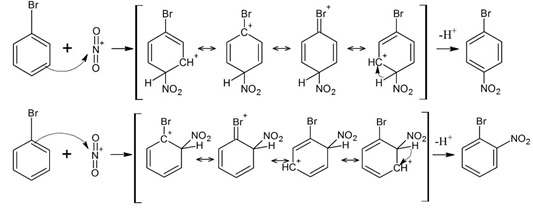
\includegraphics[width=0.8\textwidth]{img/mechanismus}
	\caption{Mechanismus der Nitrierung von Brombenzol}
	\label{fig:mechanismus}
\end{figure}
\FloatBarrier
%Ende



